\subsection{Electron Cloud Model}

The Schrödinger equation would pave the way for the electron cloud model of the atom we use today, but there has to be a little more work to be done before we can get there.
The next step in the journey relates to Heisenberg and his famous uncertainty principle.
In Heisenberg's model of the atom, he never explicitly talked about the physical position or momentum of the electron; definitely breaking with tradition. Instead, his theory focused on the observables of the electron, namely the frequency of light emitted or absorbed. He would go on to refine his uncertainty principle to state:

One can never know with perfect accuracy both of those two important factors which determine the movement of one of the smallest particles—its position and its velocity (or momentum). It is impossible to accurately determine both the position and velocity of a particle at the same instant.

\begin{flushright}--- Werner Heisenberg,\end{flushright}

Or to present the idea in math form,

\begin{align}
  \Delta x \cdot \Delta p &\geq \frac{\hbar}{2} \
\end{align}

Where $\Delta x$ stands for the uncertainty in position, $\Delta p$ stands for the uncertainty in momentum, and $\hbar$ represents the reduced Planck constant\cite{Heisenberg_1927}.

Max Born took the uncertainty principle and applied it to Schrödinger's equation, leading him to interpret $\Psi$ as a probability amplitude. Under this model, one could not know the exact positions of the electrons in an atom, but rather a probability of the electron being in a specific position at a specific time.

This can be visualized as a cloud of points surrounding the nucleus where the density of the dots indicates a higher probability of the electron being at a certain position.

\begin{figure}[H]
  % https://en.wikipedia.org/wiki/Atomic_orbital#/media/File:Hydrogen_Density_Plots.png
  \centering
  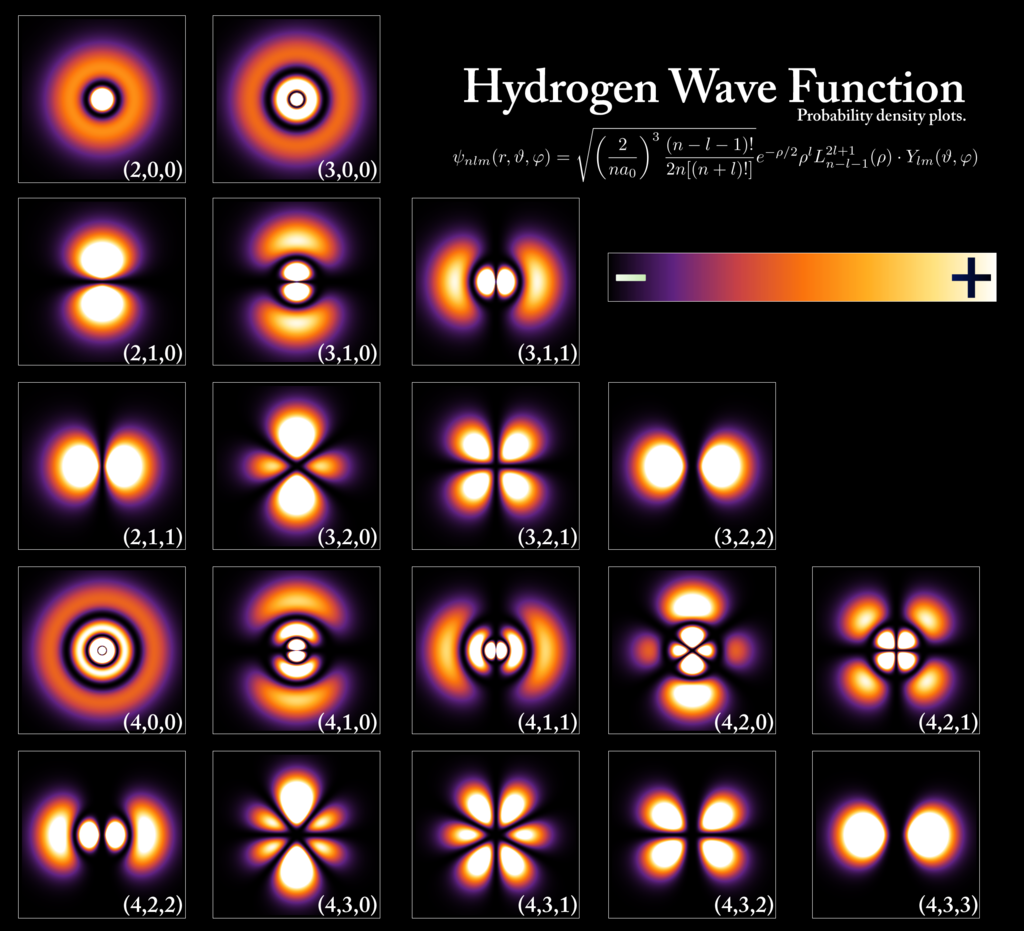
\includegraphics[width=100mm]{figures/electronCloud.png}
  \caption{Atomic orbitals of the electron in a hydrogen atom}
  \label{electronCloud}
\end{figure}

Based on this model, electrons are in a state of quantum superposition until a spatial measurement is conducted.
They don't have fixed orbits, but rather orbitals corresponding to probabilities as can be seen for the hydrogen atom in figure \ref{electronCloud}.
These orbitals surround a dense nucleus at the center of the atom.
